\documentclass[../main]{subfiles}
\begin{document}

\chapter{Introduction to Cryptography}

\section{Secret key cryptography}
We will see a first example of encryption scheme where only the sender (Alice) and the addressee (Bob) can read the plaintext with a shared key. An attacker $A$ can read the ciphertext inside the channel.
\begin{figure}[h]
    \centering
    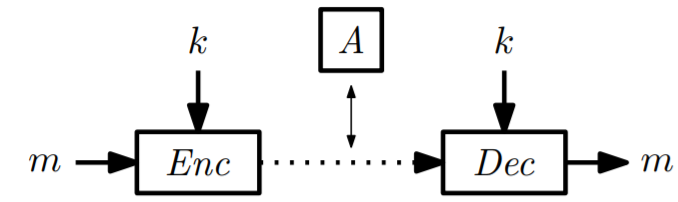
\includegraphics[width=0.5\textwidth]{images/secret_key_cryptography.png}
    \caption{Symmetric encryption scheme.}
\end{figure}
\newline
In general, an encryption scheme is defined with a triple of algorithms $(Gen, Enc, Dec)$ where:
$$Gen: 1 \rightarrow{} \mathcal{K} \quad\quad Enc: \mathcal{M} \times \mathcal{K} \rightarrow{} \mathcal{C} \quad\quad Dec: \mathcal{C} \times \mathcal{K} \rightarrow{} \mathcal{M}$$
We can assume that a scheme is correct when $Dec(Enc(m, k), k) = m$.
%----------------------------------------------------------------------------------
\section{Kerchoff’s principle}
We must assume that in every scenario the attacker $A$ know the encryption scheme and all its components, the only thing that he doesn't know is the key $k$.
We should also remember that the knowledge of $A$ can change over time and that changing the key is easy meanwhile changing the encryption scheme is much more complicated.
%----------------------------------------------------------------------------------
\section{Possible attack scenarios}
The adversary knows how the encryption scheme is defined but we are interesting in how he performs its attack and how it can act in the channel. We will study four possible attack scenarios:
\begin{itemize}
    \item \textit{Ciphertext-only attack}, the adversary $A$ knows only a certain number of cryptograms $c_1, \dotsc, c_m$ so he interferes with the communication in a passive way.
    \item \textit{Known-Plaintext Attack}, the adversary $A$ knows a certain number of pairs $(m_1, c_1), \dotsc{},(m_k, c_k)$, where $c_i$ is the cryptogram corresponding to $m_i$, it is a passive attack.
    \item \textit{Chosen-Plaintext Attack}, the adversary $A$ begins to play an active role, he can compute $Enc_k(m) = Enc(m, k)$ for messages of his own choice.
    \item \textit{Chosen-Ciphertext Attack}, the adversary $A$ participates in an even more active way in the communication, having access to an “oracle” $Deck(\cdot{})$ for decryption but obviously without having access to k.
\end{itemize}

\end{document}